\documentclass[11pt, a4paper, twoside]{article}   	% use "amsart" instead of "article" for AMSLaTeX format

\usepackage{geometry}                		% See geometry.pdf to learn the layout options. There are lots.
\usepackage{pdfpages}
\usepackage{caption}
\usepackage{minted}
\usepackage[german]{babel}			% this end the next are needed for german umlaute
\usepackage[utf8]{inputenc}
\usepackage{color}
\usepackage{graphicx}
\usepackage{titlesec}
\usepackage{fancyhdr}
\usepackage{lastpage}
\usepackage{hyperref}
\usepackage[autostyle=false, style=english]{csquotes}
\usepackage{mathtools}
\usepackage{tabularx}
% http://www.artofproblemsolving.com/wiki/index.php/LaTeX:Symbols#Operators
% =============================================
% Layout & Colors
% =============================================
\geometry{
   a4paper,
   total={210mm,297mm},
   left=20mm,
   right=20mm,
   top=20mm,
   bottom=30mm
 }	

\definecolor{myred}{rgb}{0.8,0,0}
\definecolor{mygreen}{rgb}{0,0.6,0}
\definecolor{mygray}{rgb}{0.5,0.5,0.5}
\definecolor{mymauve}{rgb}{0.58,0,0.82}

\setcounter{secnumdepth}{4}


% the default java directory structure and the main packages
\newcommand{\srcDir}{../src}
\newcommand{\imageDir}{images}
% =============================================
% Code Settings
% =============================================
\newenvironment{code}{\captionsetup{type=listing}}{}
\newmintedfile[cppSourceFile]{cpp}{
	linenos=true, 
	frame=single, 
	breaklines=true, 
	tabsize=2,
	numbersep=5pt,
	xleftmargin=10pt,
	baselinestretch=1,
	fontsize=\footnotesize
}
\newmintinline[inlineCpp]{cpp}{}
\newminted[cppSource]{cpp}{
	breaklines=true, 
	tabsize=2,
	autogobble=true,
	breakautoindent=false
}

\newcommand{\xvdash}[1]{%
  \vdash^{\mkern-10mu\scriptscriptstyle\rule[-.9ex]{0pt}{0pt}#1}%
}

% =============================================
% Page Style, Footers & Headers, Title
% =============================================
\title{Übung 3}
\author{Thomas Herzog}

\lhead{Übung 3}
\chead{}
\rhead{
\includegraphics[scale=0.10]{FHO_Logo_Students.jpg}}

\lfoot{S1610454013}
\cfoot{}
\rfoot{ \thepage / \pageref{LastPage} }
\renewcommand{\footrulewidth}{0.4pt}
% =============================================
% D O C U M E N T     C O N T E N T
% =============================================
% =============================================
% 2016.10.13: 1 
% 2016.10.14: 2
% =============================================
\pagestyle{fancy}
\begin{document}
\setlength{\headheight}{15mm}
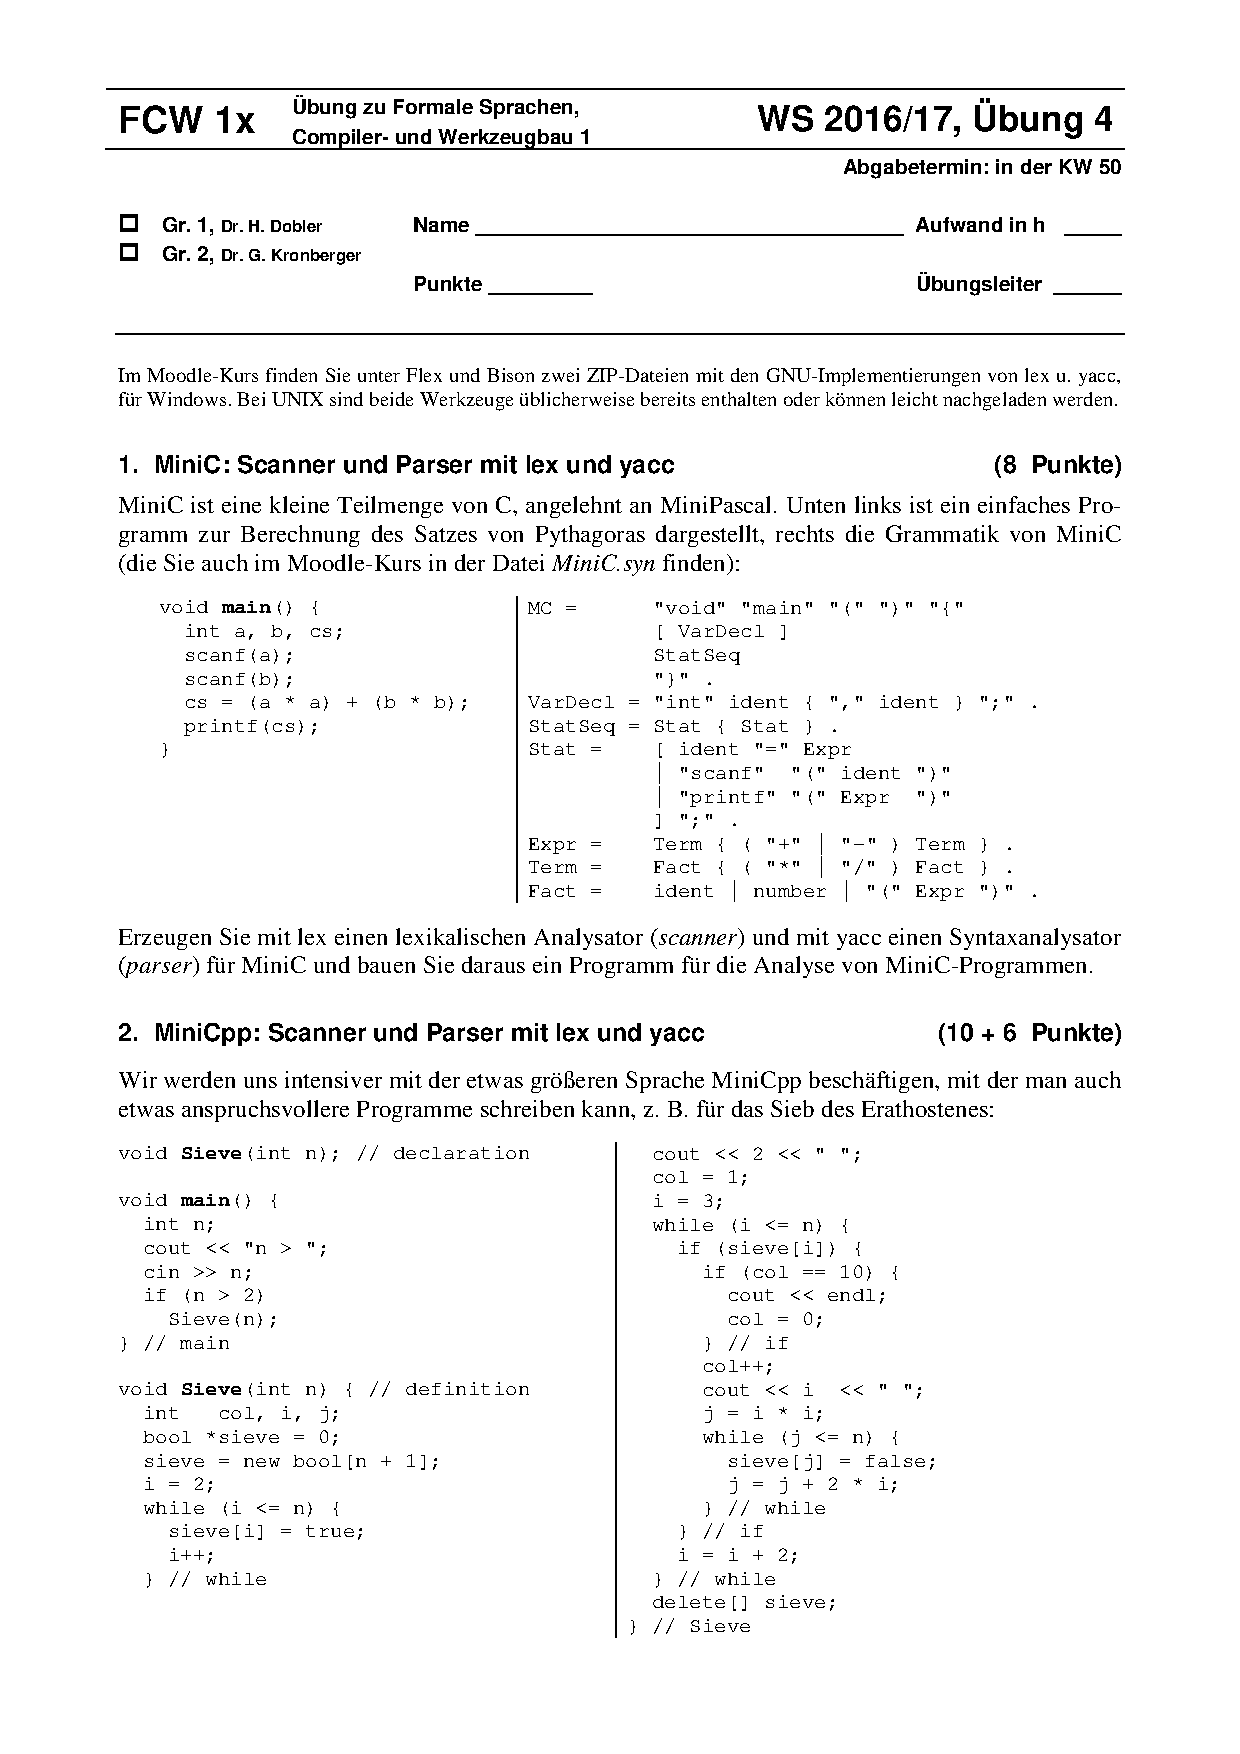
\includepdf[pages={1,2}]{Fcw1x04A.pdf}

\section{MiniC: Scanner und Parser mit lex und yacc}
\label{sec:minic}

\begin{code}
	\caption{minic.l}
	\cppSourceFile{\srcDir/MiniC/minic.l}
	\label{src:minic-l}
\end{code}

\begin{code}
	\caption{minic.y}
	\cppSourceFile{\srcDir/MiniC/minic.y}
	\label{src:minic-y}
\end{code}

\subsection{MiniC Tests}
\begin{code}
\caption{Testprogramm für Parser}
\cppSourceFile{\srcDir/MiniC/test.c}
\label{src:minic-test}
\end{code}

\begin{figure}[h]
	\centering
	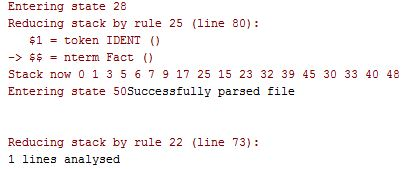
\includegraphics[scale=1]{\imageDir/minic-test.JPG}
	\caption{Ausgabe Testprogramms für Parser}
	\label{fig:minic-test}
\end{figure}
\ \newpage


\section{MiniCpp: Scanner und Parser mit lex und yacc}
\label{sec:minic}
\begin{code}
	\caption{minicpp.l}
	\cppSourceFile{\srcDir/MiniCPP/minicpp.l}
	\label{src:minicpp-l}
\end{code}

\begin{code}
	\caption{minicpp.y}
	\cppSourceFile{\srcDir/MiniCPP/minicpp.y}
	\label{src:minicpp-y}
\end{code}

\begin{code}
	\caption{Testprogramm für Parser}
	\cppSourceFile{\srcDir/MiniCPP/test.cpp}
	\label{src:minicpp-test}
\end{code}

\begin{code}
\caption{Testprogramm für Graphviz Test}
\cppSourceFile{\srcDir/MiniCPP/test2.cpp}
\label{src:minicpp-graphviz-test}
\end{code}

\subsection{MiniCPP Tests}

\begin{figure}[h]
	\centering
	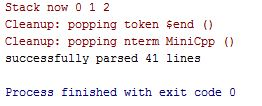
\includegraphics[scale=0.9]{\imageDir/minicpp-test.JPG}
	\caption{Ausgabe Testprogramm für den Parser}
	\label{fig:minicpp-test}
\end{figure}

\begin{figure}[h]
\centering
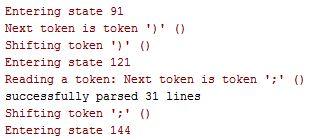
\includegraphics[scale=0.9]{\imageDir/minicpp-graphviz-test.JPG}
\caption{Ausgabe Testprogramm für Graphviz}
\label{fig:minicpp-test}
\end{figure}
\ \newpage

\begin{code}
	\caption{Generierte Graphviz Datei}
	\cppSourceFile{\imageDir/graph.gv}
	\label{src:minicpp-graphviz-test2}
\end{code}

\begin{figure}[h]
\centering
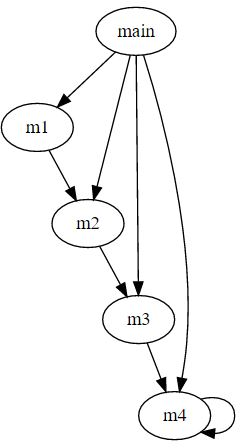
\includegraphics[scale=1]{\imageDir/miniccp-graphviz-test.JPG}
\caption{Statischer Aufrufgraph des zweiten Testprogramms}
\label{fig:minicpp-graphviz-test}
\end{figure}

 
\end{document}